%%%%%%%%%%%%%%%%%%%%%%%%%%%%%%%%%%%%%%%%%
% Journal Article
% LaTeX Template
% Version 1.4 (15/5/16)
%
% This template has been downloaded from:
% http://www.LaTeXTemplates.com
%
% Original author:
% Frits Wenneker (http://www.howtotex.com) with extensive modifications by
% Vel (vel@LaTeXTemplates.com)
%
% License:
% CC BY-NC-SA 3.0 (http://creativecommons.org/licenses/by-nc-sa/3.0/)
%
%%%%%%%%%%%%%%%%%%%%%%%%%%%%%%%%%%%%%%%%%

%----------------------------------------------------------------------------------------
%	PACKAGES AND OTHER DOCUMENT CONFIGURATIONS
%----------------------------------------------------------------------------------------

\documentclass[twoside,twocolumn]{article}

\usepackage{blindtext} % Package to generate dummy text throughout this template 

\usepackage[sc]{mathpazo} % Use the Palatino font
\usepackage[T1]{fontenc} % Use 8-bit encoding that has 256 glyphs
\linespread{1.05} % Line spacing - Palatino needs more space between lines
\usepackage{microtype} % Slightly tweak font spacing for aesthetics

\usepackage[english]{babel} % Language hyphenation and typographical rules

\usepackage[hmarginratio=1:1,top=32mm,columnsep=20pt]{geometry} % Document margins
\usepackage[hang, small,labelfont=bf,up,textfont=it,up]{caption} % Custom captions under/above floats in tables or figures
\usepackage{booktabs} % Horizontal rules in tables

\usepackage{lettrine} % The lettrine is the first enlarged letter at the beginning of the text

\usepackage{enumitem} % Customized lists
\setlist[itemize]{noitemsep} % Make itemize lists more compact

\usepackage{abstract} % Allows abstract customization
\renewcommand{\abstractnamefont}{\normalfont\bfseries} % Set the "Abstract" text to bold
\renewcommand{\abstracttextfont}{\normalfont\small\itshape} % Set the abstract itself to small italic text

\usepackage{titlesec} % Allows customization of titles
\renewcommand\thesection{\Roman{section}} % Roman numerals for the sections
\renewcommand\thesubsection{\roman{subsection}} % roman numerals for subsections
\titleformat{\section}[block]{\large\scshape\centering}{\thesection.}{1em}{} % Change the look of the section titles
\titleformat{\subsection}[block]{\large}{\thesubsection.}{1em}{} % Change the look of the section titles

\usepackage{fancyhdr} % Headers and footers
\pagestyle{fancy} % All pages have headers and footers
\fancyhead{} % Blank out the default header
\fancyfoot{} % Blank out the default footer
\fancyhead[C]{MIPS Assembler $\bullet$ November 2017 $\bullet$ Bargach Ayoub} % Custom header text
\fancyfoot[RO,LE]{\thepage} % Custom footer text

\usepackage{titling} % Customizing the title section

\usepackage{hyperref} % For hyperlinks in the PDF

\usepackage{listings} % To print code smartly

\usepackage[toc,page]{appendix} % To manage appendix

\usepackage{graphicx} % To add pictures

%----------------------------------------------------------------------------------------
%	TITLE SECTION
%----------------------------------------------------------------------------------------

\setlength{\droptitle}{-4\baselineskip} % Move the title up

\pretitle{\begin{center}\Huge\bfseries} % Article title formatting
\posttitle{\end{center}} % Article title closing formatting
\title{MIPS Assembler} % Article title
\author{%
\textsc{Ayoub Bargach} \\[1ex] % Your name, in case : \thanks{A thank you or further information}
\normalsize Grenoble INP \\ % Your institution
\normalsize https://github.com/bargacha/MIPS % Your email address
%\and % Uncomment if 2 authors are required, duplicate these 4 lines if more
%\textsc{Jane Smith}\thanks{Corresponding author} \\[1ex] % Second author's name
%\normalsize University of Utah \\ % Second author's institution
%\normalsize \href{mailto:jane@smith.com}{jane@smith.com} % Second author's email address
}
\date{\today} % Leave empty to omit a date
\renewcommand{\maketitlehookd}{%
\begin{abstract}
\noindent This documentation aim to explicit the way the MIPS assembly have been built. This project have been followed through my education in Phelma - Grenoble INP. A basic source files have been written by Francois Portet and Francois Cayre. The project goal is to build a complete assembler in C language. The biggest part is open source in my github. Due to lack of information about initial code license, formatting files have been deleted. I'm working on creating a more visual interface for education purposes. From structure to code, you will find a lot of explanation of how an assembler is built. A special thanks to all those who took time to help me when we was stucked.
\end{abstract}
}

%----------------------------------------------------------------------------------------

\begin{document}

% Print the title
\maketitle

%----------------------------------------------------------------------------------------
%	ARTICLE CONTENTS
%----------------------------------------------------------------------------------------

\section{Introduction}

\lettrine[nindent=0em,lines=3]{T} he goal of this computing project is to build an assembler for MIPS processors using C language. This assembler will be able to translate a human understandable language (Here assembler) to a machine understood language (binaries). This binaries are designed for MIPS 32 bits processors. As an input, the program takes an object file that is actually a text file. Depending on options, it will produce :

\begin{itemize}

  \item An assembly list.
  \item A binary object.
  \item An object in ELF format.

\end{itemize}

We will \textbf{not} implement all the instruction set. Indeed, the purpose is to highlight the functioning of an assembler, not to build a brand new one (gcc do it well). This project have been built in 4 deliverables (or sprints). For each one, there is a description of sprint goals, functions that must be implemented and those who are effectively implemented.




%------------------------------------------------

\section{Run and test}

To run the assembler, use makefile to compile the program (\textbf{ debug } if you want to print logs and \textbf{ release } if not). You can use some options to explicit to the program what you want as a result. It is not mandatory to use them, by default, you will get an object ELF file.

\begin{lstlisting}
./as-mips [Options ..] pathToFile
\end{lstlisting}


\begin{table}[h!]
\caption{Options}
\centering
\begin{tabular}{|l|r|}
\hline
Option & Function \\
\hline
-l & To produce an assembly list \\
-b & To produce only a binary object \\
-r & For ELF release \\
-t & To run a test \\
\hline
\end{tabular}
\end{table}

\textit{Note :} Each test is speciafied by an ID. Just fill the ID to generate the test. (Can be run either in debug and release) Please refer to appendix A to have a precise description on every test.


%------------------------------------------------

\section{The project}

\subsection{What is MIPS ?}
MIPS is a reduced instruction set computer (RISC) instruction set architecture. Designed by MIPS Technologies, it have been introduced in 1985. The philosophy of a RISC architecture is to offer a reduced -means in a single memory cycle- instruction set. It doesn't mean that there is less instruction. In fact, RISC instruction are sometimes bigger than CISC ones. RISC architectures have fixed-length instructions and simplified incoding that enable an improved code density. Also, it is based on load/store architecture that means that the result of calculations is made by specific instructions. ALU instructions mainly use general purpose registers that simplify compiler design. RISC processors solve generally an instruction in one cycle.

Like major RISC processors, MIPS are featured in a Harvard memory model that seperate physically the instruction memory from data memory that we distiguish by using directives .text and .data. Thus, changing data does not impact the code.

In this project, we aim to focus on a specific MIPS processor, the first made one. We will not be interessed in application-specific extensions such as MIPS MCU or MIPS DSP (For signal processing). The aim is to build a simple binary ELF object that can be run using MIPS I for instance. All extension that can be seen in other MIPS extension such as floating point instruction will not be handled.

The MIPS architecture is based on pipeline architecture. As a picture often speaks better than a thousand words, here a simplified drawing of the first commercialized MIPS processors R2000 :

\begin{figure}[h!]
\begin{center}
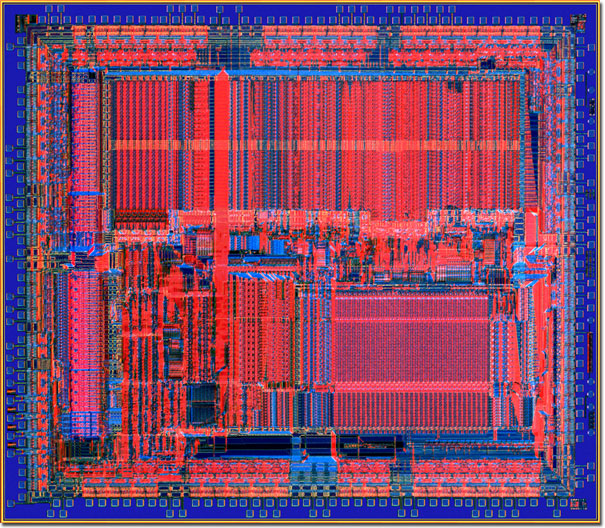
\includegraphics[width=5cm]{images/MIPS-R2000.jpg} 
\end{center}
\caption{Layout of MIPS R2000}
\label{Layout MIPS R2000}
\end{figure}

\begin{figure}[h!]
\begin{center}
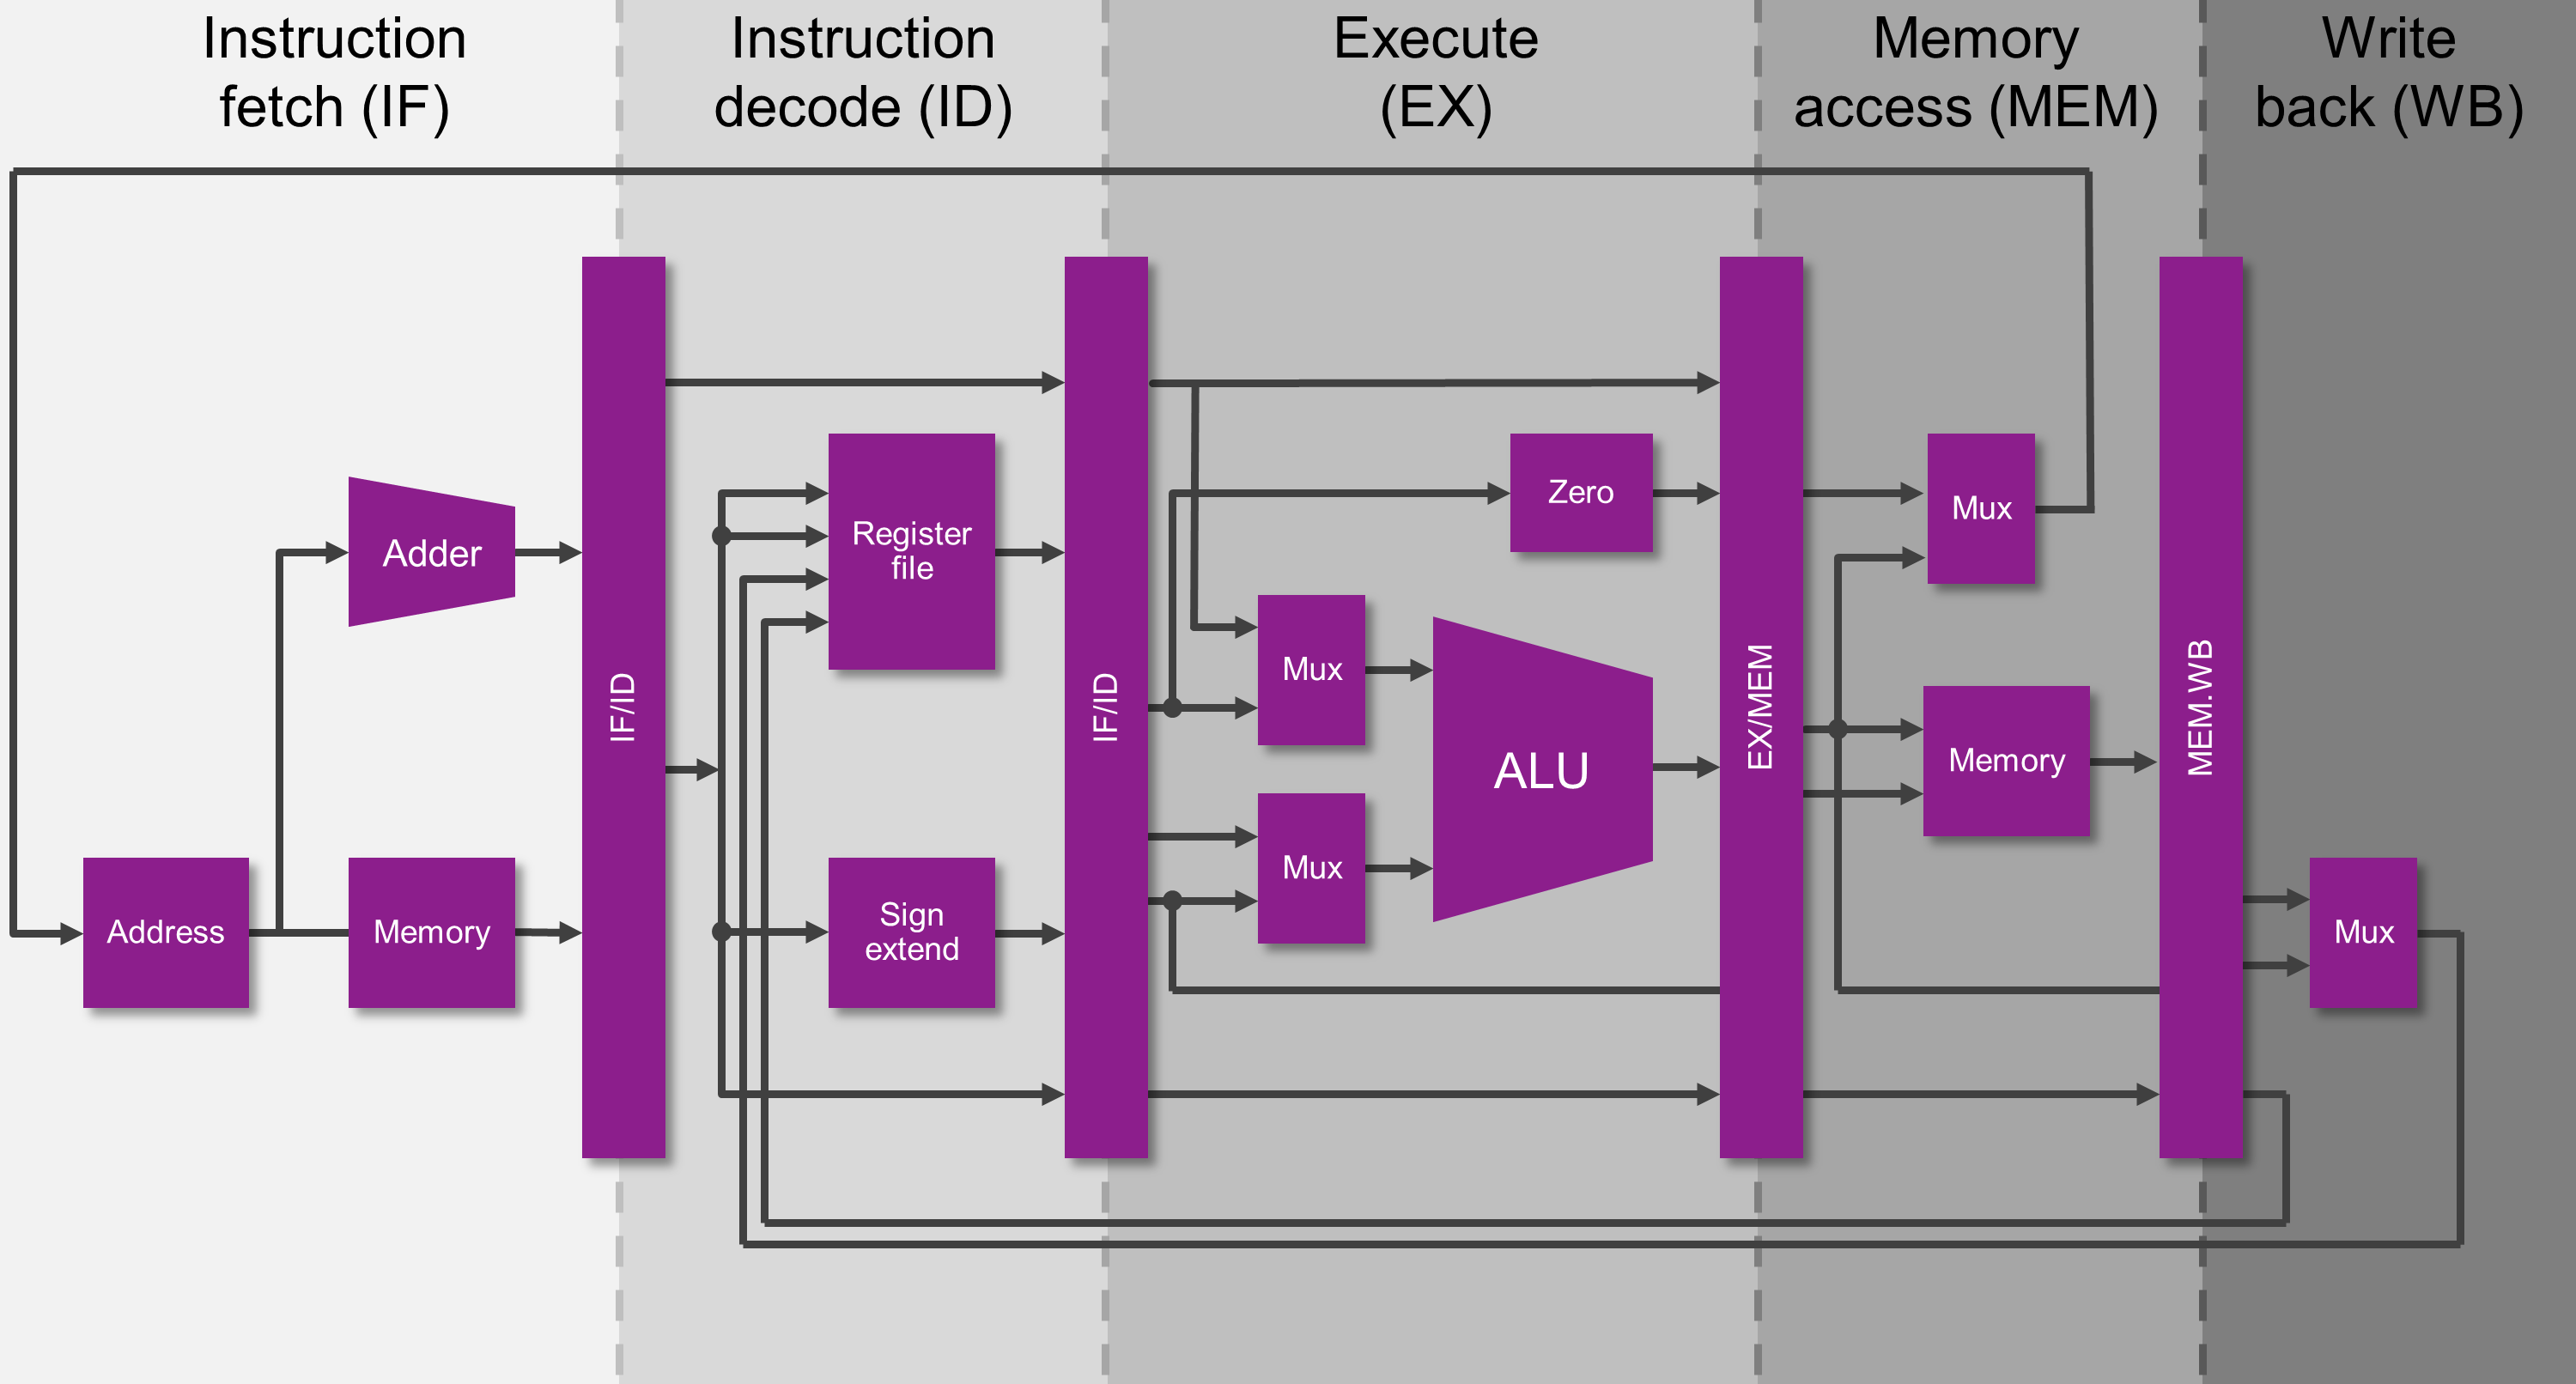
\includegraphics[width=6cm]{images/MIPS-R2000-pipeline-architecture.png} 
\end{center}
\caption{Pipeline of MIPS R2000}
\label{MIPS R2000}
\end{figure}

This pipeline is organised in several stages :

\begin{description}
 \item[ Instruction Fetch ] This stage retrieve the next instruction to decode using the program counter.
 \item[ Instruction Decode ] The retrieved instruction is decoded following the type of the instruction.
 \item[ Execute ] The instruction is executed. The execution depends on the decoded input. MUXs are used to manage the execution and control the ALU input.
 \item[ Memory access ] Give access to memory in order to load or store data in registers.
 \item[ Write back ] Upload the value of some register depending of the execution results.
\end{description}

This pipeline is the same in many RISC processors. If you are interested on how a processor is designed, here a VHDL description of an ARM processor with the same number of stages (Of course, the instruction set is completely different !) : https://github.com/bargacha/ARM-Processor

Ideally, each instruction is made in a cycle without hazards. However, when instructions depends on older ones or when branch instructions are triggered, it may have some delay.

The MIPS processor have a 4Go memory adressable by bytes. It means that incrementing Program Counter (PC) is the same as jumping 8 bits. In addition, all MIPS processors are \textit{big endian} : The high byte first, followed by the lower bytes.

\subsection{All features}

All features are recorded in this section. In order to manage correctly the project, I started by pinpoint the subject and describe what will be implemented in our basic assembler project. The main goal is to :

\begin{quotation}
 \textbf{Implement a basic MIPS assembler. As a input, it will get a standarized MIPS assembler file and should produce as an output an ELF binary file that can be executed using QEMU, an emulator for many basics processors.}
\end{quotation}

Features are :

\begin{itemize}
 \item An assembler for MIPS 32 bits microprocessor.
 \item Manage 32 General Purpose Registers with support of conventional notations (\$sp means register \$29).
 \item Main instructions are supported. The standard provided by MIPS Technologies will be followed. Please refer to InstSet.txt to see wich ones are managed. \textbf{ By following the syntax, you can add instructions directly in this file ! } Also, pseudo-instructions are implemented in the same file.
 \item Comments are managed.
 \item Main directives are managed : .text, .data, .bss, .set (only noreorder), .word ...
 \item All adressing modes will be implemented.
 \item Can take options that define wich input will be produced. (See section 'Run and Test')
 \item Can produce an assembly list that explicit each line of the source code.
 \item Can produce a binary object.
 \item Can produce an ELF binary object understood by in many OS.
 \item Using -t option can print some testing logs. No output file are produced in this case.
\end{itemize}

In addition, at the time of writing, I plan to offer some basic optimisation examples to reduce hazards in pipeline processors. To do so, please add the option -o.

\subsection{Program structure and delivrables}

This document is organised according to our professors intructions. Indeed, this project have been made in my college context. It means that code is built around deliverables to provide each 3 weeks. Here a description of each deliverable :

\begin{description}
 \item[ Deliverable 1 ] Lexical analysis. Understand the signification of each word and build a chain of lexemes.
 \item[ Deliverable 2 ] Syntaxic analysis. All instructions are fetched and decoded.
 \item[ Deliverable 3 ] Syntaxic analysis. The instructions syntax is verified and relocation inputs are generated.
 \item[ Deliverable 4 ] The outputs are generated. (Assembly list, binary object and ELF binary object)
\end{description}

The program structure is :
\begin{description}
 \item [ main.c ] The main code.
 \item [ lex.c ] Lexical analysis.
 \item [ syn.c ] Syntaxic analysis.
 \item [ eval.c ] Used in syntaxic analysis to evaluate relocation informations.
 \item [ print.c ] To generate outputs.
 \item [ functions.c ] Some useful functions.
\end{description}

For more information, please refer to the head of each source where a complete description is provided. You can also use Doxygen.



\subsection{Project management tools}
In order to keep the project organised and be able to work with other collaborators, all sources will be shared in my github. To get initial sources, here the college link : http://tdinfo.phelma.grenoble-inp.fr/

In addition, a project management tool will be used : Odoo. It is an open source tool based on kanban models. There is many tools for collaborative work. In order to reduce costs, I took a free AWS server and I implemented a basic configuration provided by http://www.pragtech.co.in/ based on ubuntu.

Finally, this report is written using LateX. The sources are also available in my github.

The program will be tested for ubuntu 16.04 and centos 6 standard configuration.

% %------------------------------------------------
% 
% Section example :
% 
% \section{Delivrable 1}
% 
% \subsection{Goals and features}
% 
% \subsection{Examples and test}

%------------------------------------------------

\section{Delivrable 1}

\subsection{Goals and features}
In this first deliverable, we aim to produce a complete lexical analysis. The main function is :

\begin{lstlisting}[language=C]
void lex_standardise( char* in, 
char* out )
\end{lstlisting}

It is responsible of the input shape and other upstream processing. It cleans redondant spaces and help to detect comments by puting a space before \#. The following function uses a simple strtok function to split a line into different word. It is mandatory to have a fully functionable function !

This function do some adjustments :

\begin{itemize}
 \item Add a space before and after chars ',', ')', '(' and '\#'
 \item No space before and only one after ':'
 \item No space after and only one before '-'
\end{itemize}

The next step concerns the construction of lexemes chain. A chain is a coding method in C to structure data. In our case, it will have this structure :

\begin{lstlisting}[language=C]
typedef struct chain_t {
  struct chain_t *next;
  union {
    struct chain_t *bottom;
    lex bottom_lex;
    inst bottom_ins;
    symbol sym;
    code c;
  }this;
} *chain;
\end{lstlisting}

In order to symplify the code, We use the same structure for all types of chains : symbol tables, code chain ... This able us to use chain elements of different types and combine them. For this purpose, we use the directive 'union' so we can manage different types of variables and reducing by the way the structure length.

For lexemes chain, here a simple drawing of how everything is working. First, the basic element of a chain :

\begin{figure}[h!]
\begin{center}
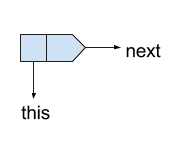
\includegraphics{images/basic_element.png} 
\end{center}
\caption{Basic element of the chain}
\label{Element}
\end{figure}

Secondly, the lexemes chain structure. Red arrow means that it points using ``struct chain\_t *bottom;''. To express the end of a chain, we use NULL operator. Black arrow contains a lexeme in this case using ``lex bottom\_lex;''.

\begin{figure}[h!]
\begin{center}
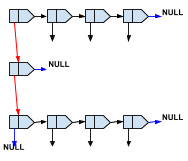
\includegraphics{images/lex_chain.png} 
\end{center}
\caption{Lexemes chain}
\label{Lex chain}
\end{figure}

To recognize lexemes, we use a FSM (finite state machine). Here another drawing that explicit the general function. For more information, the code have been commented to specify each step.

\begin{figure}[h!]
\begin{center}
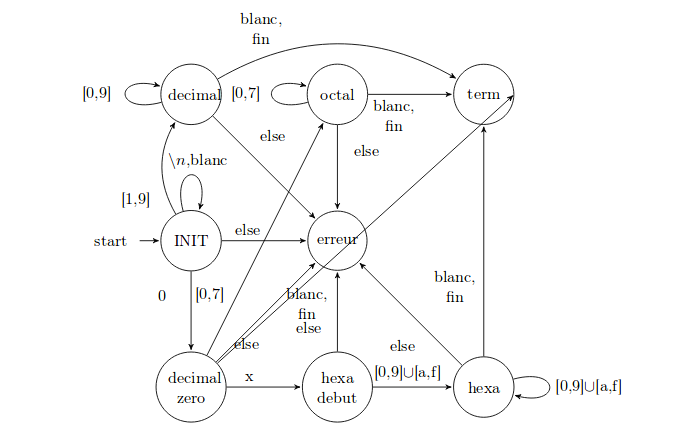
\includegraphics[width=7cm]{images/FSM.png} 
\end{center}
\caption{FSM - Credits to Francois Portet}
\label{Lex chain}
\end{figure}

In the end of this deliverable, we must have a clean collection of lexemes. It means that sometimes, we may have some errors. For example, the lexeme '0R6155' is not legal. Indeed, this syntax means that we expect an octal number and the char 'R' is not expected. However, the program understand some basic deviations such as '099' that can be translated to a Decimal number.

Thus, when a lexeme is not legal, a error is raised by a specific sentence : 'Lexical error'.


\subsection{Examples and test}

To try lex\_standardise, run test 1 using file miam.s for instance :

\begin{lstlisting}
./as-mips -t 1 tests/miam.s
\end{lstlisting}

It will print you the input and the standardised output. Normally, this function manage all basic cases. Of course, there is no further verifications in lexical analysis. It means that this function do not raise errors. It just bring an easy readable string that can be used after for further analysis.

To display lexeme chain, \textbf{run test 2}. It will print the recognized lexemes and their types.

To conclude :
\begin{itemize}
 \item A chain of lexemes is generated, it contains all relevant lexemes.
 \item We manage bad written source code by standardising it before further analysis.
 \item Comments and punctuations are ignored.
 \item FSM manages decimal, octal, hexa, labels, registers, directives and symbols.
 \item You can find all lexeme and chain functions in the file functions.c
 \item \textbf{This step is fully functional.}
\end{itemize}


%------------------------------------------------

\section{Delivrable 2}

\subsection{Goals and features}
In this deliverable, we start by generating the instruction set. The instruction set is the list of all instructions that are taken into account by our program. In MIPS context, there 3 kinds of instructions :

\begin{figure}[h!]
\begin{center}
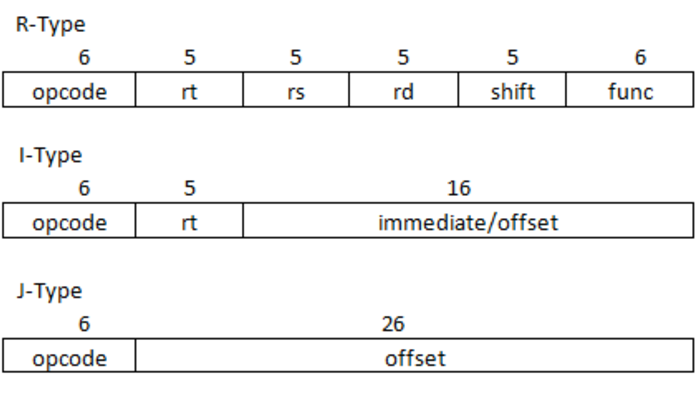
\includegraphics[width=7cm]{images/instType.png} 
\end{center}
\caption{Instruction types from researchgate.net}
\label{instType}
\end{figure}

Also, we note that for I-type instructions, there is 2 ways to code it in MIPS assembly code (depending on the instruction), for example : 

\begin{itemize}
 \item For ADDI instruction : ADDI \$rt, \$rs, immediate
 \item For Load instruction : LW \$rt, offset(\$rs)
\end{itemize}

For this reason, we have in fact 4 type of grammatical sentences in MIPS Assembly language : R, I (for ADDI), J and IB (for LW). I and IB is a distinction who have nothing to do with the binary decoding. It will just help us to optimize the code.

The list of this instructions are set in the file ``instSet.txt``. The file can be modified to add other primary instructions (To add for example floating points instructions). The file have been designed as follows :

\begin{lstlisting}
OP OPCODE TYPE OPERAND SPECIAL
SRL 000010 0 0111 rs=00001
\end{lstlisting}

\begin{itemize}
 \item OP is the name of operation
 \item OPCODE, the code translate in binary
 \item TYPE, decribe the type defined in global.h by ''enum \{R, I, J, IB\};``
 \item OPERAND, expected operands. For R-type, 0111 means 0 rs 1 rt 1 rd 1 sa. So we need rt, rd and sa to execute the instruction. If not the assembler fail !
 \item SPECIAL, for future purposes. If an operand is not defined, you can set it (rs=00001). It is very useful to contruct pseudo-instructions.
\end{itemize}

Using this simple implementation, we build the instSet table using the structure inst.

\begin{lstlisting}[language=C]
typedef struct inst_t {
  char name[16];
  char op[16];
  int type;
  char operand[8];
  char special[STRLEN];
} *inst;
\end{lstlisting}

For performance purposes, we use a simple hash function knowing that our table does not exceed hundred lines. Furthermore, the instruction ID will be built by concatenating/decaling ASCII value and calculate it modulo 1000.

Thus, for ADD, Hash function will calculate : $( A + D << 1 + D << 2 ) \% 1000$. Also, the program analyse automatically if there is any collision. If there is one, he raises an error.

In fact, we add all instructions included pseudo-instruction in instSet.txt. If you had more instructions, be aware that you will have to change certainely the hash function. But before, try changing modulo int.

\textit{Note} : Please respect the instSet syntax in order to avoid any problem. a single double space may occur in unpredication errors.

The next stage is to generate the symbol table. We use the same structure as lexeme chain. we will get something that is near to this illustration :

% Ajouter une illustration de la structure de SymTab

After that, we range through all lines of lexeme chain to analyse it, in other word, to make the syntaxic analysis. Each step is described in syn.c. The ''main`` function is fetch(). it uses different functions from decodeInstruction() to decodeDirective(). We ''fetch`` each line and generate the next elements of code chain, symbol chain and relocation chain. In the end of this process, we will run a final function named eval. This function will make the final links between symtab and undefined yet relocations. (But all of this will be made in the third deliverable)


\subsection{Examples and test}
To print all the instruction tab, please run test 3. It will also print you the ID of the symbol. This test is useful is you want to add instructions.  You can also update hash function in order to make it more robust :

\begin{lstlisting}[language=C]
int hash( char * s, int modulo ) {
  int i =0;
  int result = 0;

  while ( s[i] != '\0' ) {
    result = result + ( s[i] << i);
    i++;
  }
  
  return result % modulo;
}
\end{lstlisting}

To conclude :
\begin{itemize}
 \item All instruction types are managed : R, I and J.
 \item A ``virtual'' type have been added, IB. It manages I instruction of this shape : LW \$6, 200(\$7).
\end{itemize}


%------------------------------------------------

\section{Delivrable 3}

\subsection{Goals and features}
In this part, we aim to manage all the final functionalities. We must properly generate the symbol Table, so it had to be optimized and robust. Thus, if the symbol table is changed, the relocation table must be also changed.

Relocation entries should be generated. Final verifications and decode will be made, especially for relocations. For instance, a BEQ instruction need a decoded offset. In a first sight, the instruction is decoded without adding any offset. So, if no related symbol is found after, that means that the instruction will keep an offset of zero.

\subsection{Examples and test}

%------------------------------------------------

\section{Delivrable 4}

\subsection{Goals and features}
In the end of this step, the program wil be able to generate a fully functional ELF object file.
As it have been specified in former section, there is 3 types of different outputs :

\begin{description}
 \item[List mode] In this mode, we generate the assembly list. It explicit each line of source code with the equivalent decode binary code. You will also find symbols and relocations tables.
 \item[Object mode] Before each section, we put the lengh of input code. For section .bss, only the lengh will be added.
 \item[ELF mode] An understandable object file, used by many major OS, focusing on a minimal implementation.
\end{description}


\subsection{Examples and test}


%----------------------------------------------------------------------------------------
%	REFERENCE LIST
%----------------------------------------------------------------------------------------

\begin{thebibliography}{99} % Bibliography - this is intentionally simple in this template

% \bibitem[Figueredo and Wolf, 2009]{Figueredo:2009dg}
% Figueredo, A.~J. and Wolf, P. S.~A. (2009).
% \newblock Assortative pairing and life history strategy - a cross-cultural
%   study.
% \newblock {\em Human Nature}, 20:317--330.

\bibitem[Wikipedia, 2017]{RISC}
\newblock Reduced instruction set computer

\bibitem[Wikipedia, 2017]{MIPS}
\newblock MIPS architecture

\bibitem[Wikipedia, 2017]{RISC}
\newblock 

\end{thebibliography}

%----------------------------------------------------------------------------------------

\appendix
\section{All test functions by ID}

\begin{table}[!h]
\caption{Tests by ID}
\centering
\begin{tabular}{|p{2cm}|p{2cm}|}
\hline
ID & Description \\
\hline
1 & Compare input and output of lex\_standarise function \\
\hline
2 & Dump the lexeme chain ( to validate the first deliverable ) \\
\hline
3 & Print instruction table \\
\hline
\end{tabular}
\end{table}


% \section{Title of Appendix B}
% % the \\ insures the section title is centered below the phrase: Appendix B
% 
% Text of Appendix B is Here

\end{document}